\section{Exercise 2: Tracers of deep ocean circulation change}
\label{sec:E2}

\subsection{Question 1}
\label{sec:Q2.1}
See Figure \ref{fig:age_depth}

\begin{figure}[!htbp]
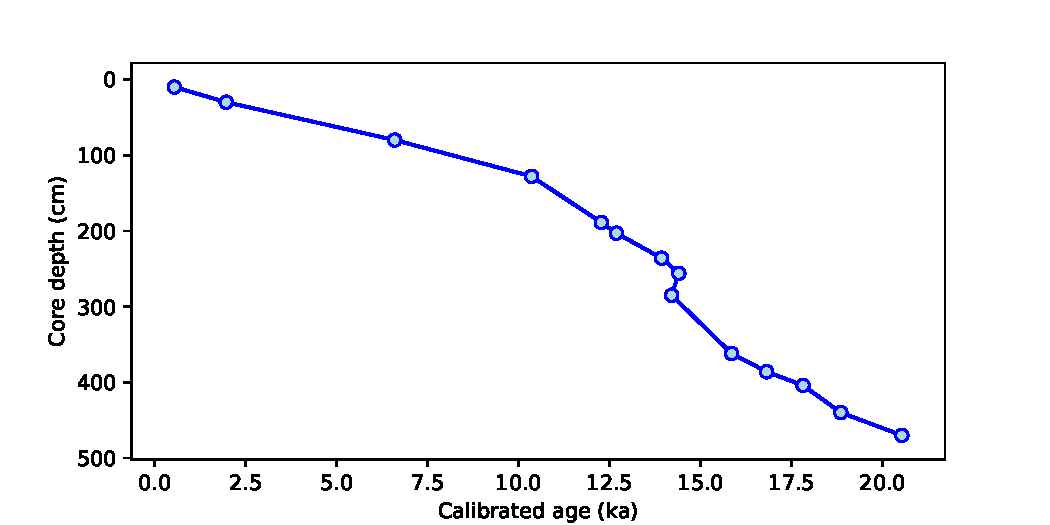
\includegraphics[width=\textwidth]{img/line_age_depth.pdf}
    \caption{Planktic foraminifera calibrated age against depth in sediment core OCE-326-GGC14, on the Laurentian fan.}
        \label{fig:age_depth}
\end{figure}

\subsection{Question 2}
\label{sec:Q2.2}

\begin{figure}[!htbp]
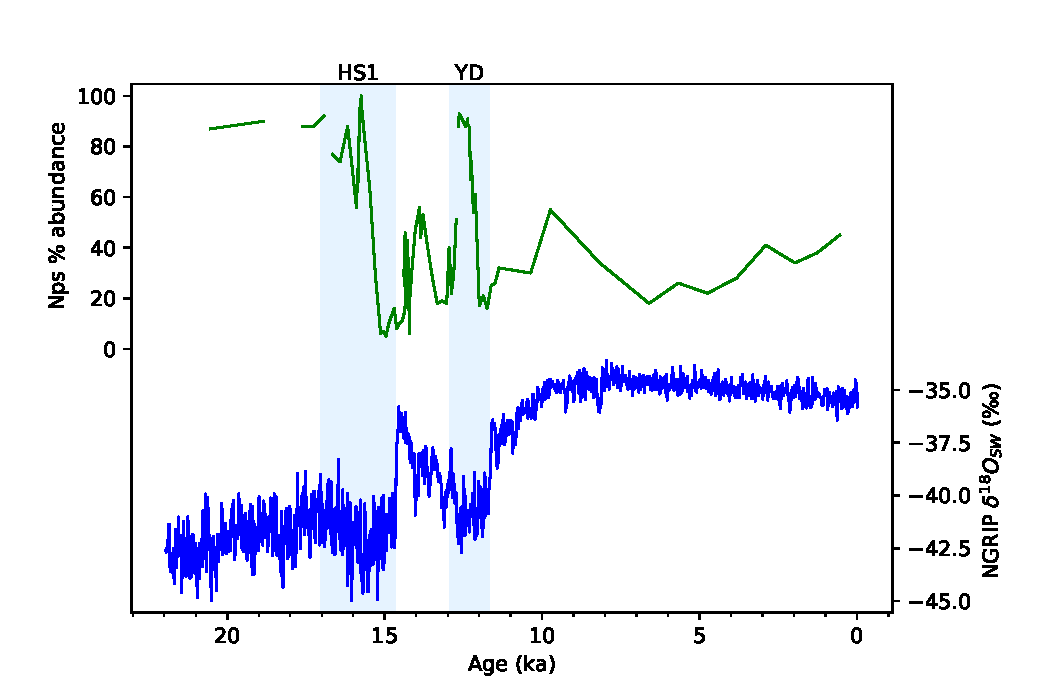
\includegraphics[width=\textwidth]{img/timeseries_nps_ngrip}
    \caption{Time series of abundance of planktic foraminifera \emph{N. pachyderma} sinistral (\emph{Nps}) in OCE-326-GGC14 (top) and oxygen isotope excursion in Greenland ice core NGRIP (bottom).}
        \label{fig:nps_ngrip}
\end{figure}

Figure \ref{fig:nps_ngrip} shows a strong antiphase relationship between \emph{Nps} abundance in the North Atlantic and \delO{} in Greenland, and both record abrupt climate cooling during the HS1 and YD stadials.
While changes in the latter appear to lag those in the former by approximately 0.5--1 ka, there is uncertainty in the calibration of foraminiferal \fC{} radiocarbon dates due to measurement error and, in particular, the assumption of a constant 400 year radiocarbon reservoir age --- a value that was likely higher during stadial events due to decreased ocean ventilation \parencite{bard1994north, hughen2004marine04}.

            
\subsection{Question 3}
\label{sec:Q2.3}
\begin{figure}[p]
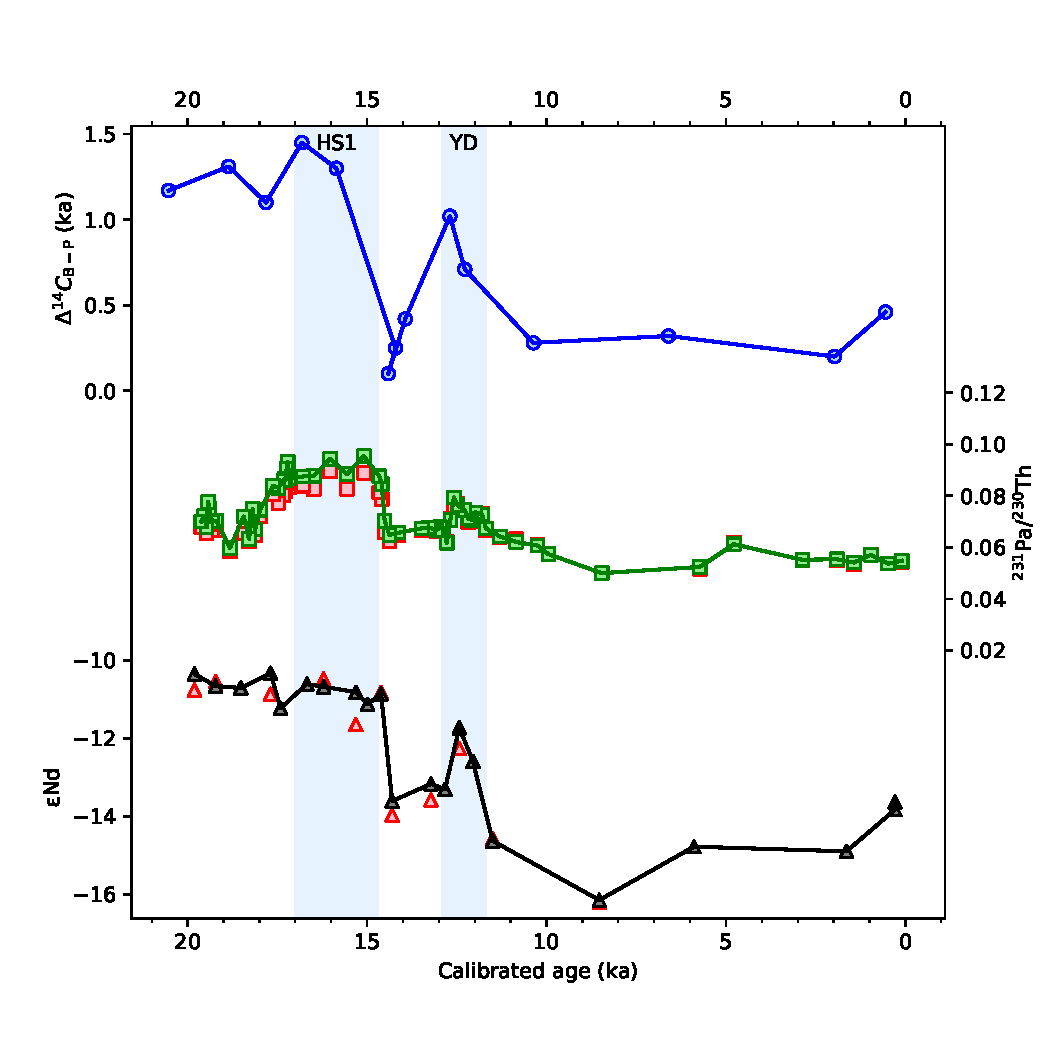
\includegraphics[width=\textwidth]{img/timeseries_B-P_PaTh_eNd}
    \caption{Time series of benthic--planktic foraminifera \fC{} ventilation age difference in OCE-326-GGC14 (top);
             $^{231}$Pa/$^{230}$Th ratio in calculated against $^{238}$U (green) and $^{232}$U (red) OCE326-GGC5 core on Bermuda rise \parencite[data from][]{mcmanus2004collapse};
             Neodynium isotopic ratio excursion in unclean foraminifera (black) and reductively cleaned fish debris (red) from OCE326-GGC6 sediment core on Bermuda Rise (bottom) \parencite[data from][]{roberts2010synchronous}.}
            \label{fig:bp_path_end}
\end{figure}
The benthic--planktic foraminifera \fC{} offset (Figure \ref{fig:bp_path_end}, top) is considerably larger at LGM, HS1 and YD than during the BA and the Holocene.
Since \fC{} of a water mass effectively records the ventilation age (i.e. time since last exposure at the surface) \parencite{lynch2014tracers}, these results indicate that the North Atlanticwas highly stratified during the cold periods, with younger northern sourced waters displaced in the deep ocean by the intrusion of more ancient waters of southern origin.
This supports evidence for the slowdown or shutoff of NADW formation during these cold periods, allowing Antarctic Bottom Water to fill the global abyssal basins \parencite{boyle1985comparison, bard1994north, thornalley2011deglacial}.
Likewise, the rapid rejuvenation of deep waters at the HS1--BA and YD--Holocene transitions shown in the \fC{} time series indicates rapid resumption of the contemporary (warm) mode ocean overturning circulation.

\subsection{Question 4}
\label{sec:Q2.4}

